\documentclass{beamer}
\usetheme{simple}
\usepackage[brazil]{babel}
\usepackage[utf8]{inputenc} 
\usepackage{lmodern}
\usepackage{ragged2e}
\usefonttheme[onlymath]{serif} 
\usepackage[scale=2]{ccicons}

\usepackage{graphicx,hyperref,url,pgfplots}
\usepackage{amsmath} 
\usepackage{array,booktabs}
\usepackage{bibentry}
%\usepackage[alf,abnt-etal-list=0,abnt-etal-cite=3]{abntex2cite}
\usepackage[normalem]{ulem} 
\pgfplotsset{compat=1.13}  

\setbeamercovered{invisible} 
% \newcommand{\pausar}{\pause}
\newcommand{\pausar}{""}
\newcommand{\df}[1]{\,\mathrm{d}#1}
\newcommand{\parcial}[3]{\dfrac{\partial^{#1}#2}{\partial #3^{#1}}}

\usepackage{tikz}
\usepackage{xcolor}
\usetikzlibrary{scopes}
\usepackage{verbatim}
\usetikzlibrary{patterns}


\usepackage{listings}
	\definecolor{codegreen}{rgb}{0,0.6,0}
	\definecolor{codegray}{rgb}{0.5,0.5,0.5}
	\definecolor{codepurple}{rgb}{0.58,0,0.82}
	\definecolor{backcolour}{rgb}{0.92,0.92,0.92}
	\lstset{language=Python, 
	backgroundcolor=\color{backcolour},   
	commentstyle=\color{codegreen},
	keywordstyle=\color{magenta},
	numberstyle=\tiny\color{codegray},
	stringstyle=\color{codepurple},
	basicstyle=\fontsize{8}{11}\ttfamily,
	frame=lines,
%	numbers=left,
	tabsize=2,
	morekeywords={models, lambda, forms}}



% --------------------------------------------------------------------------------------------

\title{Robótica Móvel}
\subtitle{Apresentação da Disciplina}
\date{\today}
\author[Jeferson José de Lima]{
  \textbf{Professor}: Jeferson José de Lima}
\institute[UTFPR-PB]{Departamento de Informática (DAINF)}

\begin{document}
\maketitle
\justify


\begin{frame}{Informações Úteis}
	\begin{block}{Material disponível em:}
		\begin{enumerate}
			\item Moodle - Robótica Móvel
			\item \href{https://gitlab.com/cursoseaulas/robotica-movel/-/wikis/home}{https://gitlab.com/cursoseaulas/robotica-movel/-/wikis/home}
		\end{enumerate}
	\end{block}
	\begin{block}{Dinâmica de Aula}
		\begin{enumerate}
			\item \textbf{Aulas Teóricas}: \textcolor{red}{Segunda-feira}
			\item \textbf{Aulas Práticas}: \textcolor{blue}{Sexta-feira}
		\end{enumerate}
	\end{block}
	\begin{block}{Requisitos da Disciplina}
		\begin{itemize}
			\item Teoria de Controle
			\item Eletrônica I
			\item Noções básicas de Mecânica
			\item Linguagem de Programação - \textbf{Python} e \textbf{C++}
		\end{itemize}
	\end{block}
\end{frame}


\begin{frame}{Expectativa - Robótica Móvel?}
\end{frame}


\begin{frame}[c]{Ementa da Disciplina}
	\framesubtitle{Robótica Móvel}

	\begin{block}{}
		\begin{itemize}
			\item \textbf{Pré-requisitos}: Sistema de Controle 1 (SC25CP), Eletrônica A (EL25CP).
			\item \textbf{Carga horária}: 60ha
			\item \textbf{Objetivos}: Apresentar conceitos, problemas e soluções para o desenvolvimento de sistemas com robôs móveis, enfatizando a autonomia, inteligência e a navegação e mapeamento simultâneos.
			\item \textbf{Ementa}: Introdução à robótica móvel. Percepção e ação. Ambientes de simulação.
			      Paradigmas de controle. Localização e mapeamento. Planejamento e navegação.
		\end{itemize}
	\end{block}
\end{frame}


\begin{frame}[t]{Robótica Móvel - Mercado de Trabalho}
	\framesubtitle{Alguns exemplos}

	\begin{enumerate}
		\item \href{https://www.indeed.com/q-Slam-Engineer-jobs.html}{Slam Engineer}
		\item \href{https://www.indeed.com/q-Autonomous-Driving-Engineer-jobs.html}{Autonomous Driving Engineer}
		\item \href{http://wiki.ros.org/Jobs}{ROS Engineer}
	\end{enumerate}
\end{frame}


\begin{frame}[c]{Ementa da Disciplina}
	\framesubtitle{Robótica Móvel}
	\begin{block}{Introdução a Robótica Móvel}
	\end{block}

	\begin{itemize}
		\item Tipo de Modelos:
		      \begin{itemize}
			      \item Modelo Cinemático;
			      \item Modelo Dinâmico;
		      \end{itemize}
	\end{itemize}
	\begin{center}
		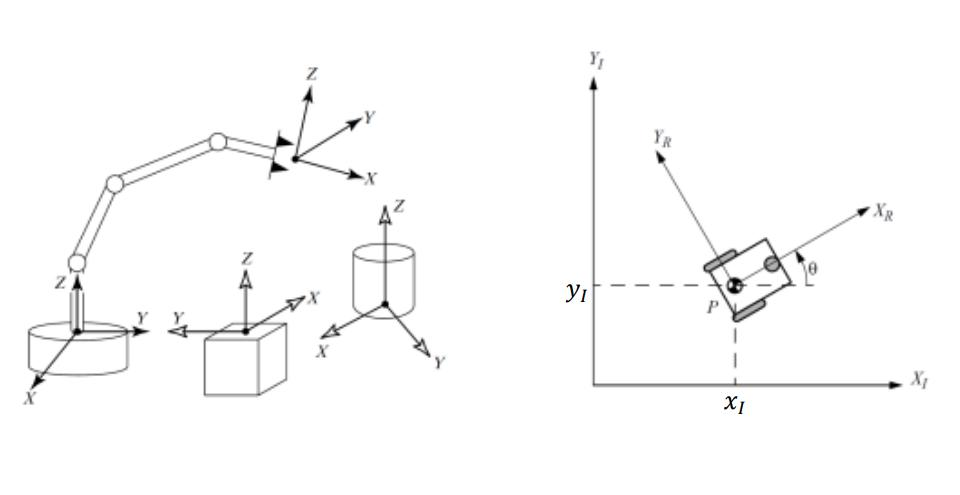
\includegraphics[width=0.8\textwidth]{./images/mecanismos.jpg}
	\end{center}
\end{frame}


\begin{frame}[c]{Ementa da Disciplina}
	\framesubtitle{Robótica Móvel}
	\begin{block}{Introdução a Robótica Móvel}
	\end{block}
	\begin{itemize}
		\item Bibliografia Referências
	\end{itemize}
	\begin{columns}[c]
		\begin{column}{0.5\textwidth}
			\center
			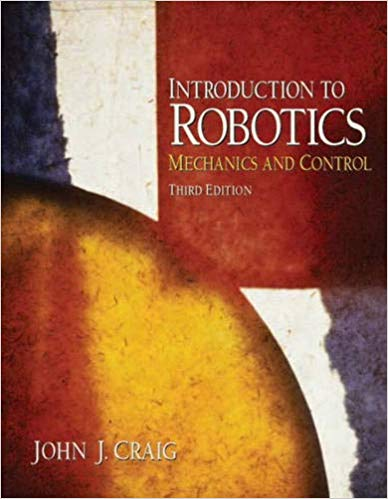
\includegraphics[width=0.7\textwidth]{./images/livro6}
		\end{column}
		\begin{column}{0.5\textwidth}
			\center
			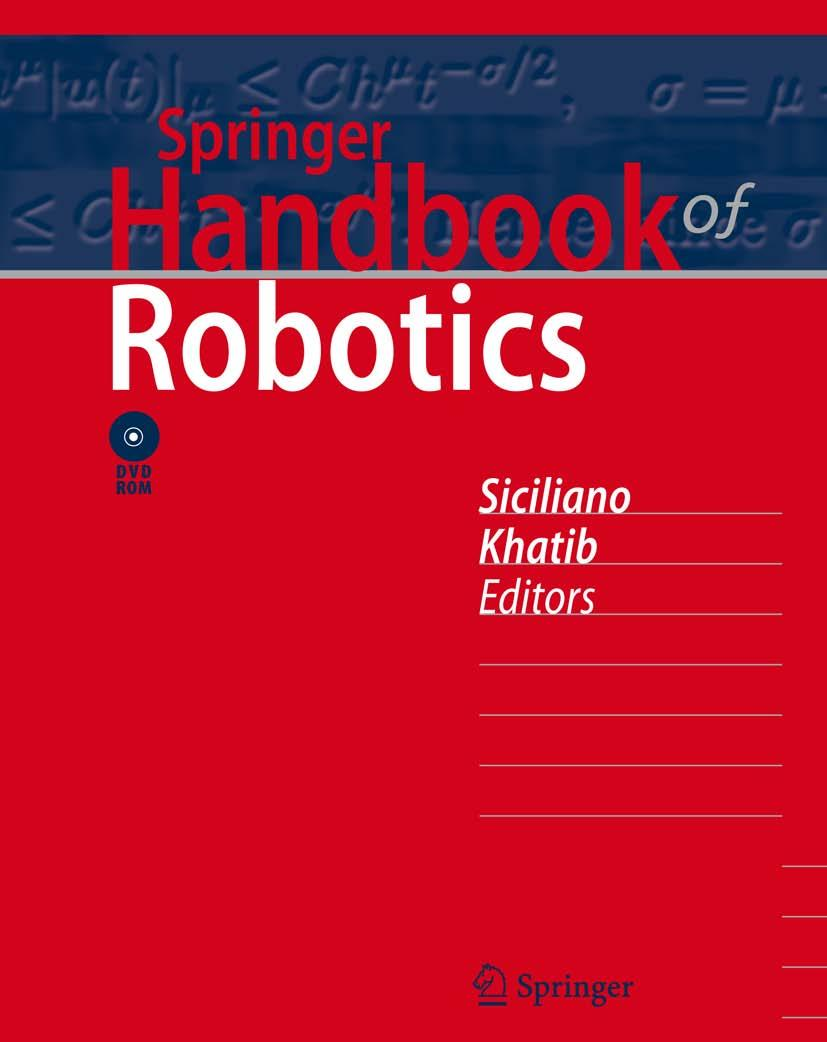
\includegraphics[width=0.7\textwidth]{./images/livro5}
		\end{column}
	\end{columns}
\end{frame}



\begin{frame}[t]{Ementa da Disciplina}
	\framesubtitle{Robótica Móvel}
	\begin{block}{Percepção e Ação}
	\end{block}
	\begin{center}
		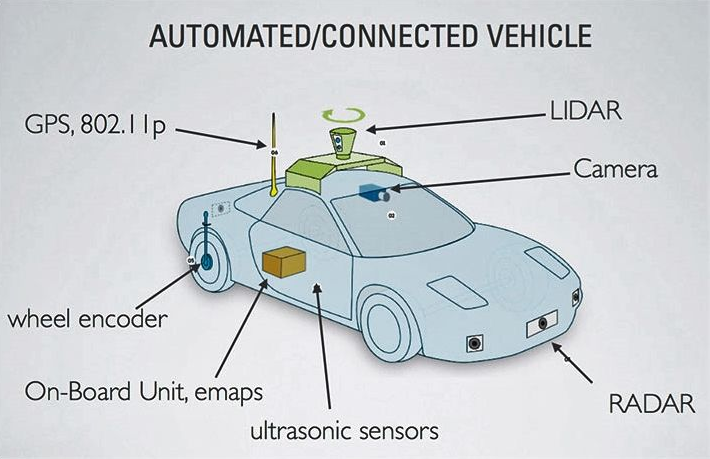
\includegraphics[width=0.6\textwidth]{./images/autonomous-car.png}

		fonte \footnote{https://edisciplinas.usp.br/course/view.php?id=72434}
	\end{center}
\end{frame}

\begin{frame}[t]{Ementa da Disciplina}
	\framesubtitle{Robótica Móvel}
	\begin{block}{Percepção e Ação}
	\end{block}
	\begin{itemize}
		\item Sensores (Ultrasom, LIDAR, Camera Stereo ...) \pausar
		\item Algoritmos para Fusão de Sensores \pausar
		\item Atuadores (Motor CC, Encoders, ...)
	\end{itemize}
\end{frame}


\begin{frame}[t]{Ementa da Disciplina}
	\framesubtitle{Robótica Móvel}
	\begin{block}{Percepção e Ação}
	\end{block}
	\begin{center}
		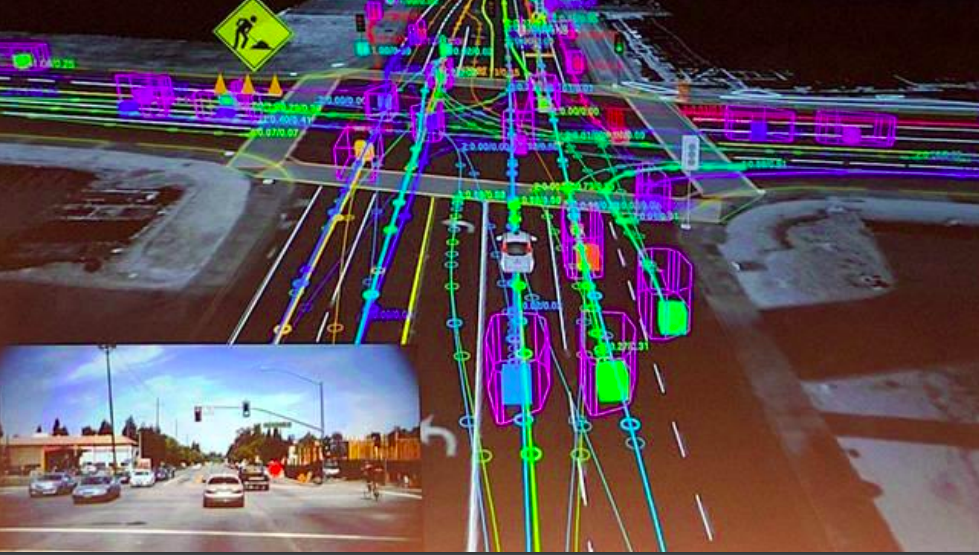
\includegraphics[width=0.9\textwidth]{./images/autonomous-car_2.png}
	\end{center}
\end{frame}


\begin{frame}[t]{Ementa da Disciplina}
	\framesubtitle{Robótica Móvel}
	\begin{block}{Percepção e Ação}
	\end{block}
	\begin{itemize}
		\item Bibliografia Referências
	\end{itemize}
	\begin{columns}[c]
		\begin{column}{0.5\textwidth}
			\center
			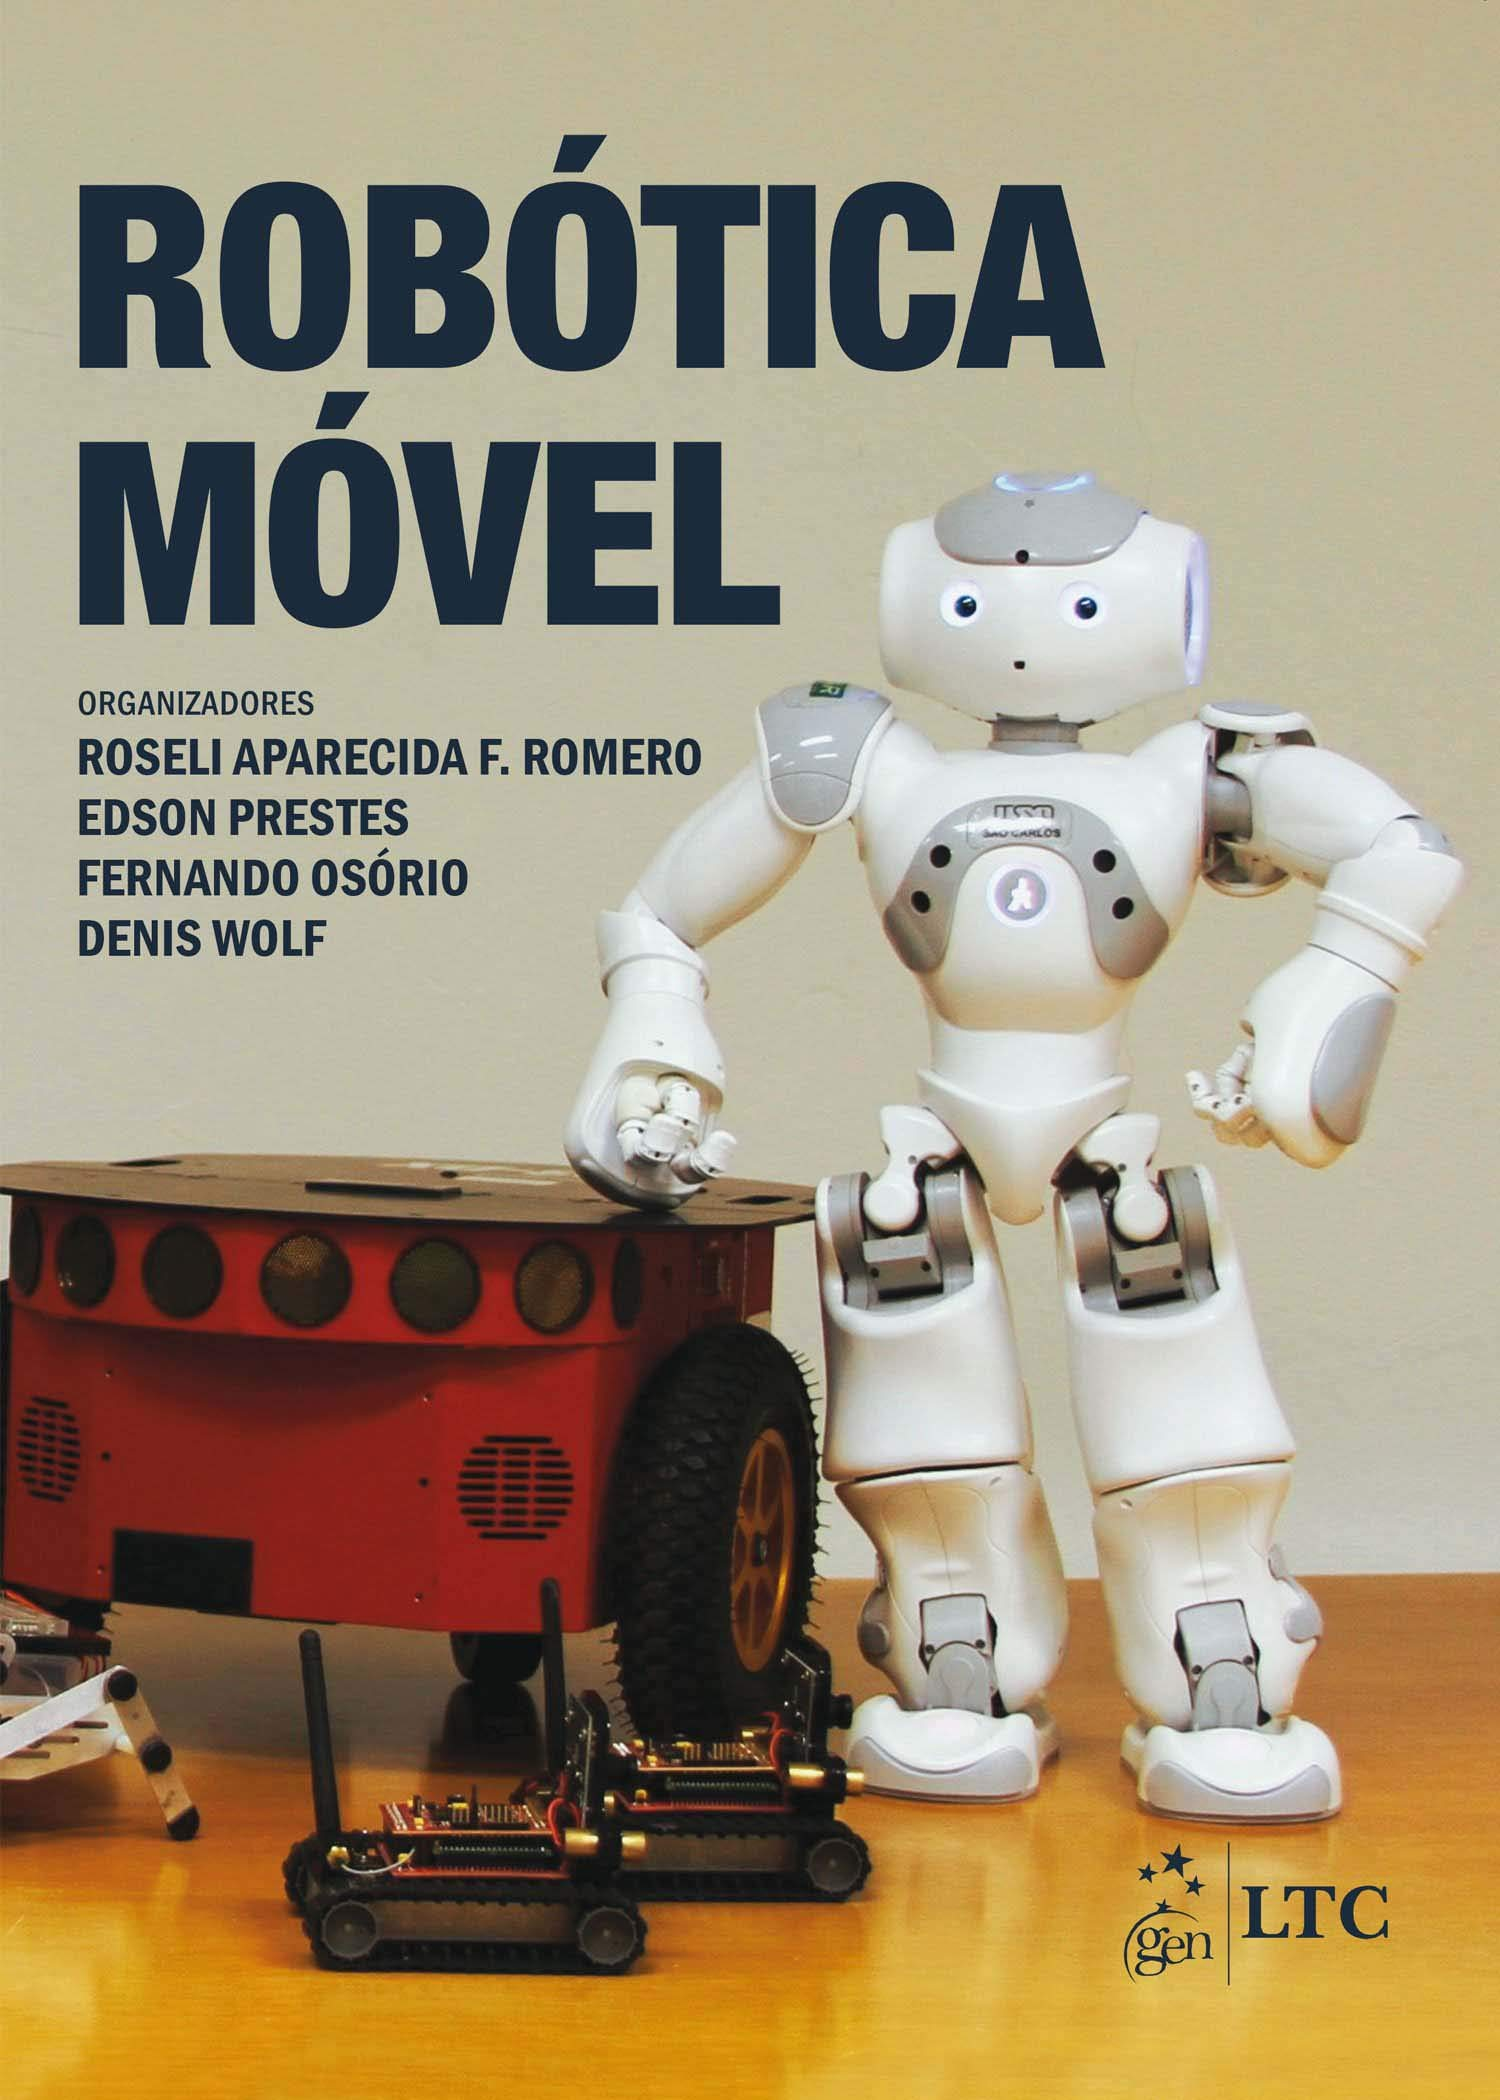
\includegraphics[width=0.7\textwidth]{./images/livro9}
		\end{column}
		\begin{column}{0.5\textwidth}
			\center
			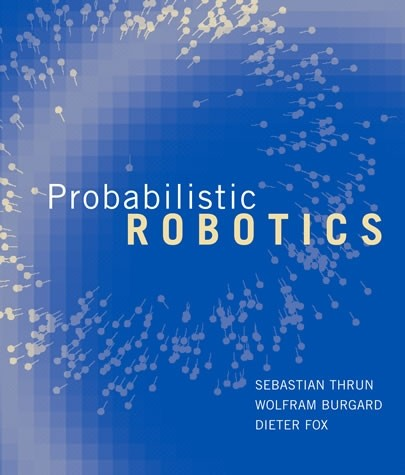
\includegraphics[width=0.7\textwidth]{./images/livro2}
		\end{column}
	\end{columns}
\end{frame}

 
\begin{frame}[t]{Ementa da Disciplina}
	\framesubtitle{Robótica Móvel}
	\begin{block}{Paradigmas de Controle}
	\end{block}
	\begin{itemize}
		\item Revisão Controle Clássico
		\item Controle Moderno
		\item Controle Ótimo
	\end{itemize}
\end{frame}


\begin{frame}[c]{Ementa da Disciplina}
	\framesubtitle{Robótica Móvel}
	\begin{block}{Paradigmas de Controle}
	\end{block}
	\begin{itemize}
		\item Bibliografia Referências
	\end{itemize}
	\begin{columns}[c]
		\begin{column}{0.5\textwidth}
			\center
			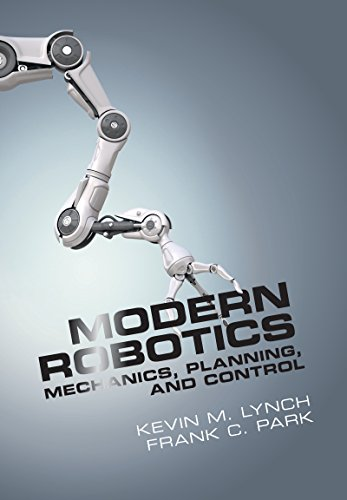
\includegraphics[width=0.7\textwidth]{./images/livro3}
		\end{column}
		\begin{column}{0.5\textwidth}
			\center
			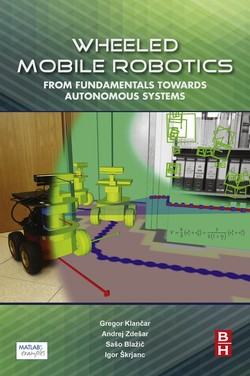
\includegraphics[width=0.7\textwidth]{./images/livro4}
		\end{column}
	\end{columns}
\end{frame}



\begin{frame}[t]{Ementa da Disciplina}
	\framesubtitle{Robótica Móvel}
	\begin{block}{Ambiente de Simulação}
	\end{block}
	\begin{itemize}
		\item  Robot Operating System (ROS)
		      \begin{center}
			      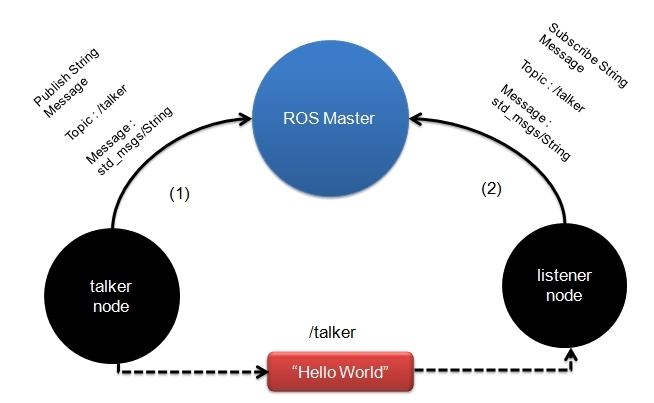
\includegraphics[width=0.7\textwidth]{./images/ros_msgs.png}
		      \end{center}
	\end{itemize}
\end{frame}



\begin{frame}[t]{Ementa da Disciplina}
	\framesubtitle{Robótica Móvel}
	\begin{block}{Ambiente de Simulação}
	\end{block}

	\begin{itemize}
		\item  Robot Operating System (ROS)
		      \begin{center}
			      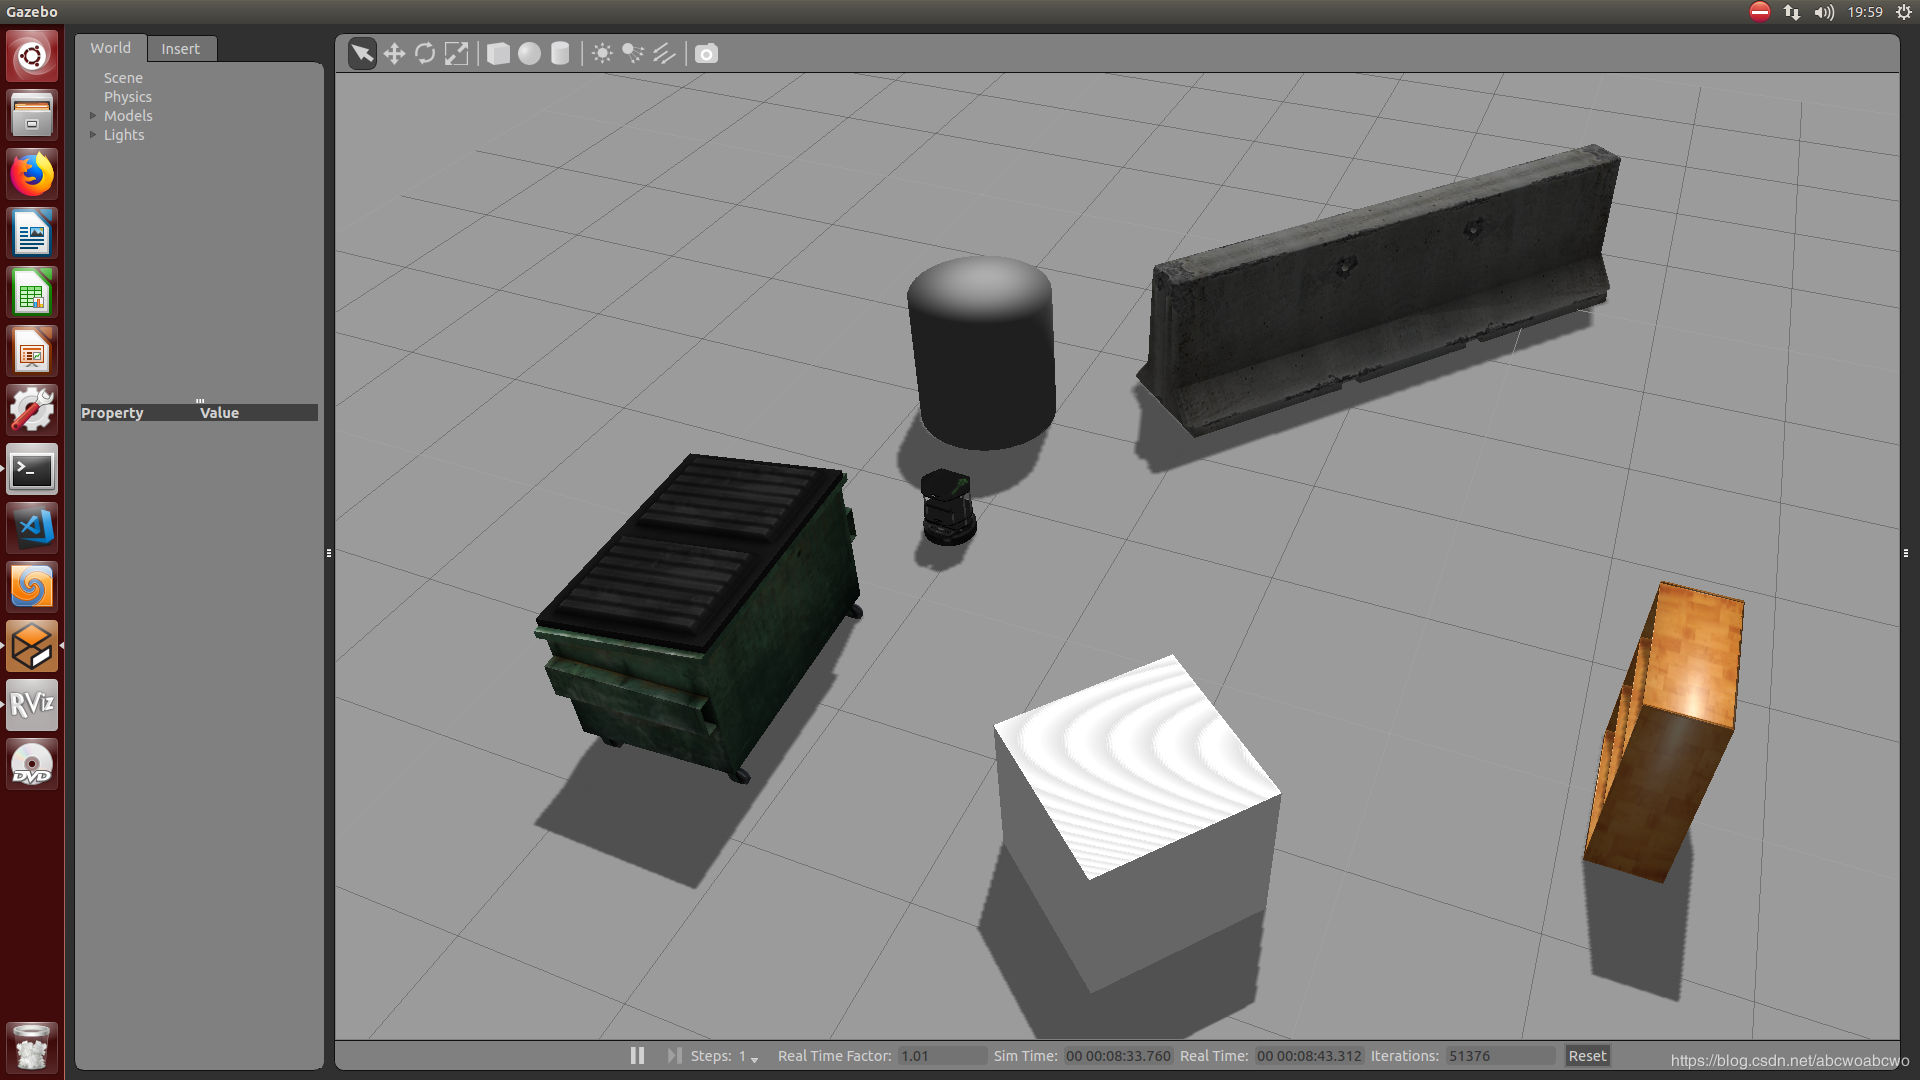
\includegraphics[width=0.7\textwidth]{./images/ros_example.png}
		      \end{center}
	\end{itemize}
\end{frame}




\begin{frame}[t]{Ementa da Disciplina}
	\framesubtitle{Robótica Móvel}
	\begin{block}{Ambiente de Simulação}
	\end{block}

	\begin{itemize}
		\item  Robot Operating System (ROS)
		      \begin{center}
			      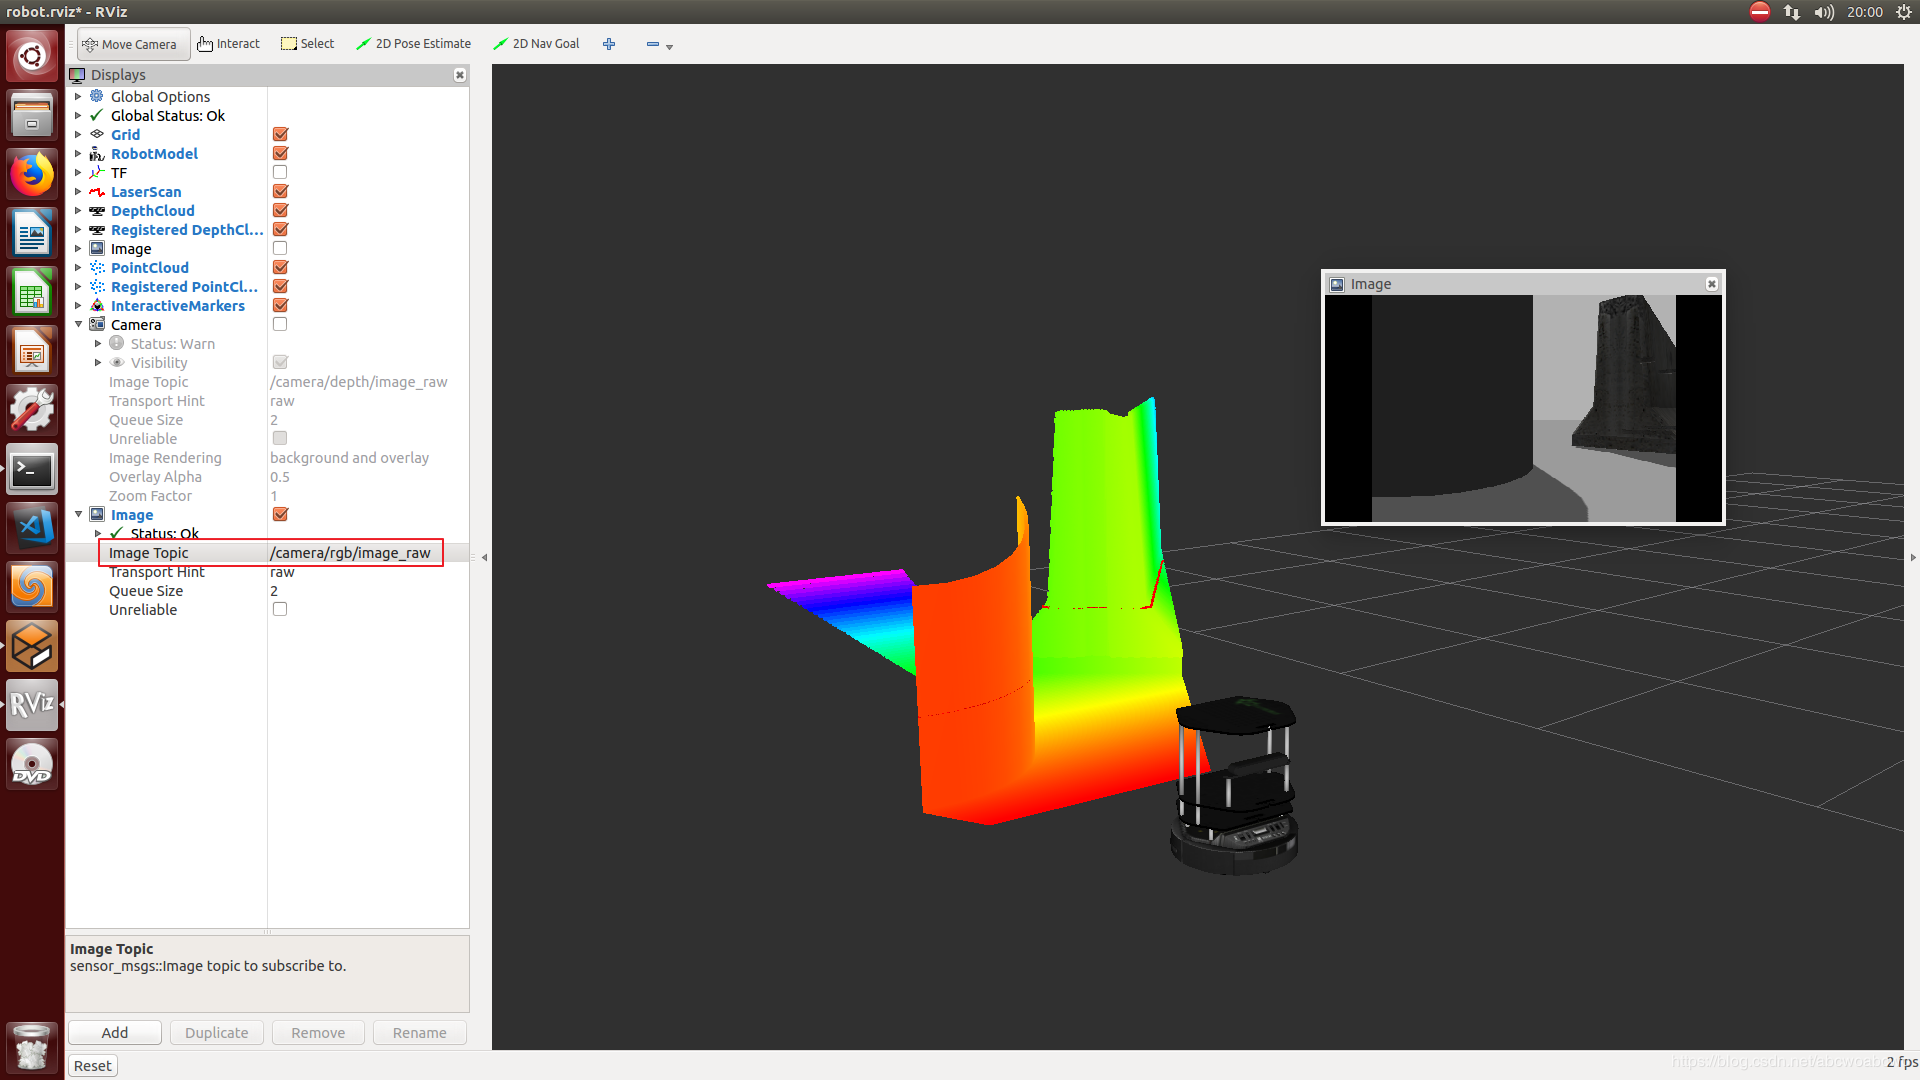
\includegraphics[width=0.7\textwidth]{./images/ros_example_2.png}
		      \end{center}
	\end{itemize}
\end{frame}


\begin{frame}[t]{Ementa da Disciplina}
	\framesubtitle{Robótica Móvel}
	\begin{block}{Ambiente de Simulação}
	\end{block}
	\begin{itemize}
		\item Bibliografia Referências
	\end{itemize}
	\begin{columns}[c]
		\begin{column}{0.5\textwidth}
			\center
			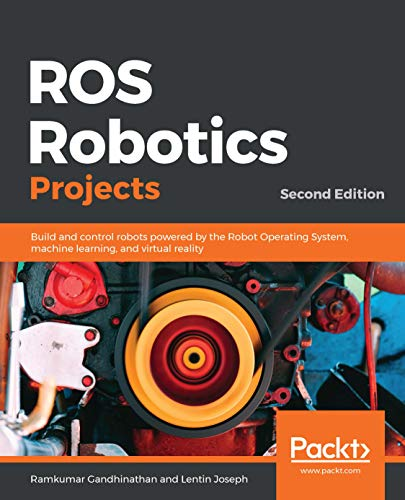
\includegraphics[width=0.7\textwidth]{./images/livro7}
		\end{column}
		\begin{column}{0.5\textwidth}
			\center
			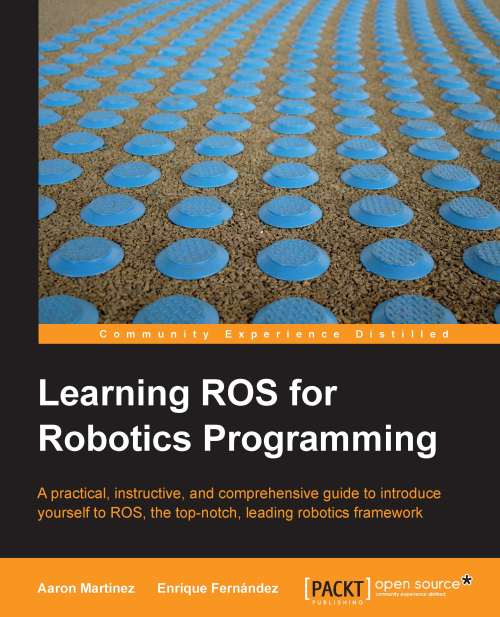
\includegraphics[width=0.7\textwidth]{./images/livro8}
		\end{column}
	\end{columns}
\end{frame}


\begin{frame}[c]{Ementa da Disciplina}
	\framesubtitle{Robótica Móvel}
	\begin{block}{Localização e Mapeamento}
	\end{block}
	\begin{center}
		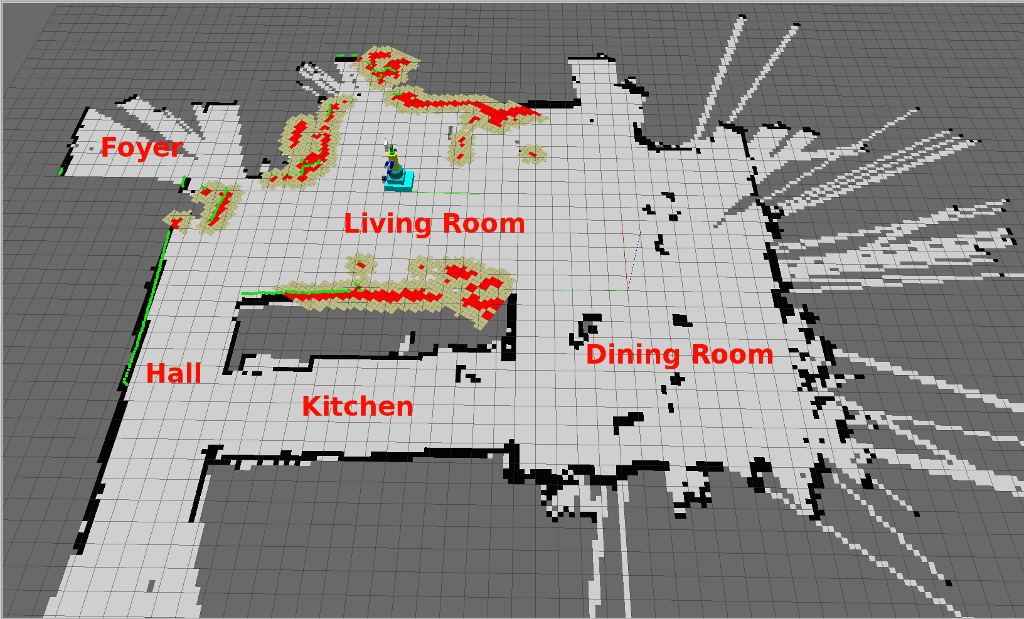
\includegraphics[width=0.7\textwidth]{./images/slam-example.png}
	\end{center}
\end{frame}


\begin{frame}[c]{Ementa da Disciplina}
	\framesubtitle{Robótica Móvel}
	\begin{block}{Localização e Mapeamento}
	\end{block}
	\begin{itemize}
		\item Bibliografia Referências
	\end{itemize}
	\begin{columns}[c]
		\begin{column}{0.5\textwidth}
			\center
			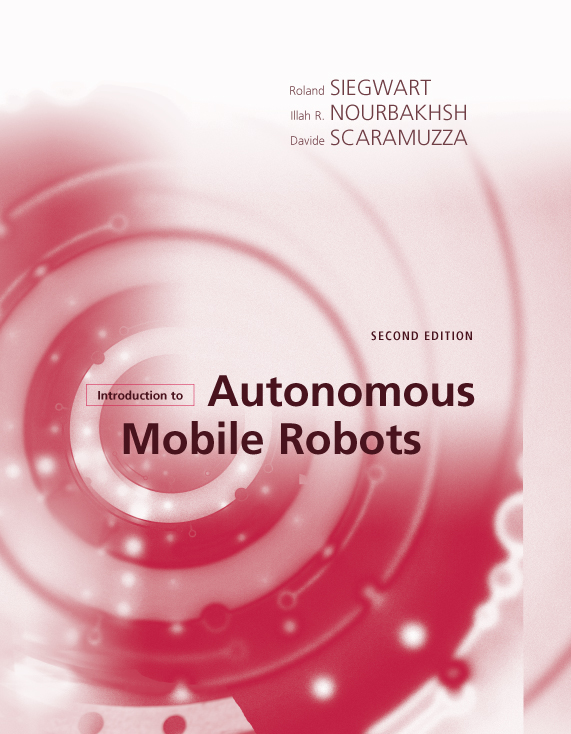
\includegraphics[width=0.7\textwidth]{./images/livro1}
		\end{column}
		\begin{column}{0.5\textwidth}
			\center
			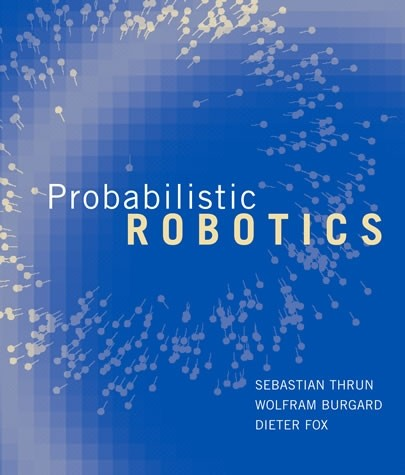
\includegraphics[width=0.7\textwidth]{./images/livro2}
		\end{column}
	\end{columns}
\end{frame}


\begin{frame}{Métodos de Avaliação}
	\begin{block}{Avaliações}
		\begin{itemize}
			\item Apenas um projeto!
		\end{itemize}
		\begin{enumerate}
			\item Desenvolvimento do Projeto Prático
			      \begin{itemize}
				      \item Direção Livre - FPV
				      \item Controle e Telemetria
				      \item Mapeamento e Localização
			      \end{itemize}
			\item Relatórios
		\end{enumerate}
	\end{block}
	\begin{block}{Peso das Avaliações}
		\begin{tabular}{lll}
			\hline
			$N_1$ & = Projeto Fase 1 * 0,7 & + Exercício/Relatório * 0,3 \\
			$N_2$ & = Projeto Fase 2 * 0,7 & + Exercício/Relatório * 0,3 \\
			$N_3$ & = Projeto Fase 3 * 0,8 & + Exercício/Relatório * 0,2 \\
			\hline
		\end{tabular}
	\end{block}
\end{frame}



% \begin{frame}[t, allowframebreaks]
% 	\frametitle{Referências}
% 	\bibliography{../template-beamer/reflatex/reflatex.bib}
% \end{frame}

\end{document}


% https://ethz.ch/content/dam/ethz/special-interest/mavt/robotics-n-intelligent-systems/rsl-dam/documents/RobotDynamics2016/0-introduction.pdf
